\newpage

\subsection{Montaža stročnic}
Stroj deluje na principu kratkostružnih stročnic. Zato vsebuje le eno stročnico,
ki jo je potrebno zamenjati. Ob menjavi je potrebno tudi preveriti pritisk
stročnice, ki se nastavlja z matico. Če je pritisk prevelik, se stročnica veliko
hitreje obrabi in tudi pušča odtise na izdelku. Če pa je premajhen, pa obstaja možnost,
da podajalec potisne palico preko stročnice, ta se lahko zatakne med
premikajoče dele, uniči rezalne plošlice ali zlomi svedre.

Ko se ta nastavi, je potrebno prilagoditi krivuljo, ki nadzira odpiranje in
zapiranje stročnice. Krivulja nam stročnico odpre, za tem se celoten zadnji suport
pomakne nazaj za dolžino kosa, kjer se palica ponovno vpne. Medtem podajalec
skozi celoten cikel potisne palico ob odrezni nož, da se ob premiku suporta ne premakne.

Potrebno je še izračunat čas, ki nam je na voljo za preprijem stročnice.
Ta se zračuna tako, da se od časa cikla odšteje ves skupni čas, potreben
za obdelavo, in sicer po spodnji Enačbi \ref{eq:13}:

\begin{equation}
	\label{eq:13}
	\begin{split}
		t_c &= t_{r1+r2} + t_{cent} + t_{vrt} + t_{odr} \\
		t_c &= 0.75\ s + 0.95\ s + 3.8\ s + 4.5\ s = 10\ s
	\end{split}
\end{equation}

Za vpetje in razpetje stročnice potrebuje stroj približno 0.2 s, za premik
suporta, pa približno 0.5--0.8s. Ker je skupen čas za obdelavo kosa
enak času enega obrata krivuljne gredi, bo potrebno nekatere obdelave
nastaviti, da se prekrivajo med sabo. Npr. v našem primeru je možno
nastaviti, da se čas pobiranja robov in centriranja prekriva ter
nam omogoča ravno dovolj časa za cikel vpetja.

Stroj GM127 uporablja stročnico, ki jo je možno izdelati tudi na stružnici, z dimenzijami, prikazanimi na Sliki \ref{slika_strocnice}.

\begin{figure}[H]
	\begin{center}
		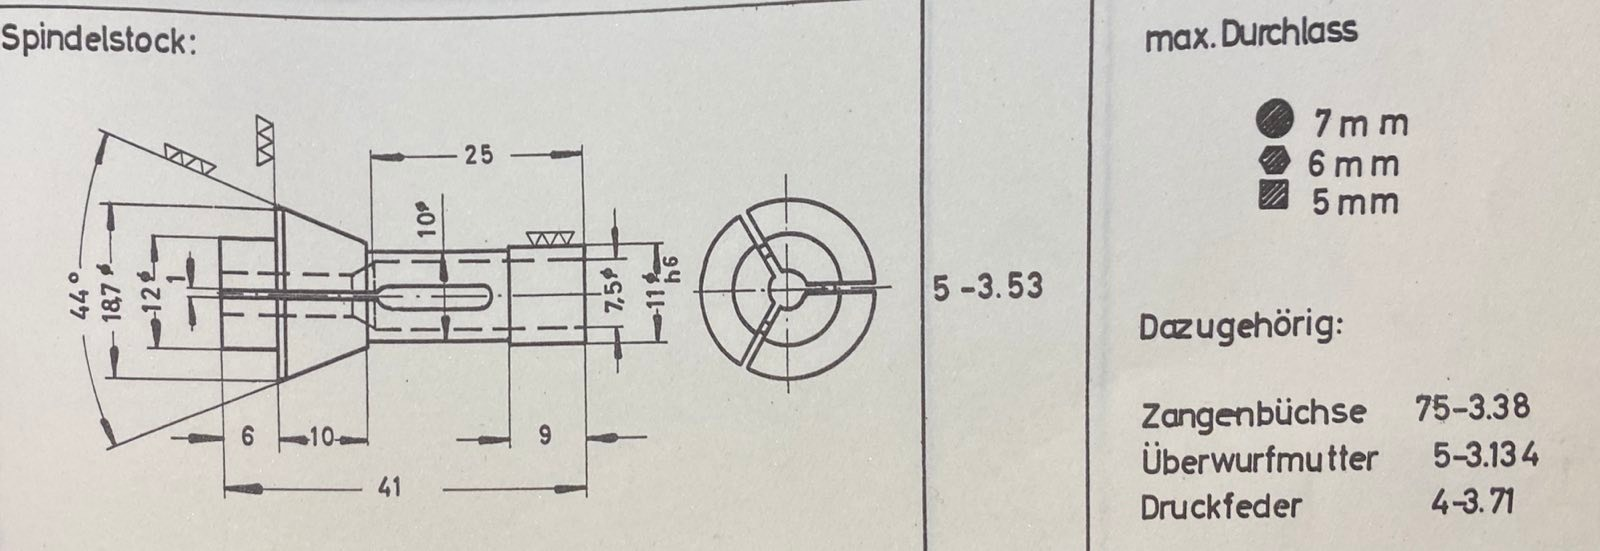
\includegraphics[width=\linewidth]{slika_strocnice.jpg}
		\caption{Slika dimenzij stročnice iz priročnika
			stroja Gauthier GM127 pod prilogo VI
			\cite{gauthier}}
		\label{slika_strocnice}
	\end{center}
\end{figure}

Stročnica vpne material zaradi sprednjega konusa, na katerega
pritisne posebna puša z nasprotno postruženim konusom. Sprednji
del stročnice je fiksiran z matico, ki preprečuje aksialni pomik,
kadar jo puša pritisne. Sistem je zelo zanimiv, saj imamo dve
puši znotraj cevi, ena je premična, druga pa fiksna. Fiksna puša
vodi material iz podajalca skozi celotno vreteno in ima tudi
ležišče, kamor se stročnica prilega. Premična puša pa preko
posebnih vpenjalnih prstov prenese silo iz krivulje na stročnico.